\documentclass[11pt]{report}
\usepackage{pgf}
\usepackage{tikz}
\usetikzlibrary{arrows,automata}
\usepackage[utf8]{inputenc}
 \usepackage{listings}
 \usepackage{color}
 \usepackage{fancyhdr}
 \usepackage{graphicx}
 \usepackage{amsmath}
\pagestyle{fancy}
 \usepackage{comment} 
 \usepackage[top=2cm, bottom=2cm, left=2cm , right=2cm]{geometry}
\begin{center}
 \lhead{Louis Caron \\ Océane DUBOIS}
 \rhead{NF16 - TP03 - Listes chainées}
 \rfoot{}
 \end{center}



\definecolor{dkgreen}{rgb}{0,0.6,0}
\definecolor{gray}{rgb}{0.5,0.5,0.5}
\definecolor{mauve}{rgb}{0.58,0,0.82}

\lstset{frame=tb,
  language=c,
  aboveskip=3mm,
  belowskip=3mm,
  showstringspaces=false,
  columns=flexible,
  basicstyle={\small\ttfamily},
  numbers=none,
  numberstyle=\tiny\color{gray},
  keywordstyle=\color{blue},
  commentstyle=\color{dkgreen},
  stringstyle=\color{mauve},
  breaklines=true,
  breakatwhitespace=true,
  tabsize=3
}

 
%Gummi|065|=)
\title{\textbf{NF16 - TP03 - Listes chainées}
\author{Louis Caron \\ Océane DUBOIS\\}
\date{}}

\begin{document}

\maketitle

\newpage

\section{Presentation}

Le but de se TP est de se familiariser avec les listes chaînées. On cherchera donc à implémenter différentes fonctions permettant à l'utilisateur de créer des éléments, créer des listes chaînées, insérer des éléments dans ses listes, supprimer des éléments de ces listes, supprimer des listes, supprimer des éléments, fusionner des listes ensemble .... 

En C il n'existe pas de type défini permettant de gérer des listes, contrairement à d'autres languages de plus hauts niveaux. 

C'est donc notre but de créer d'abord des éléments puis des listes composées de ces différents éléments.

\section{Fonctions implémentées}

Nous avons commencé par implémenter la structure Element comme suivant 

\begin{lstlisting}
struct Element {
	char valeur[20];
	struct Element* suivant;
	struct Element* precedent;
};
typedef struct Element T_Element;
\end{lstlisting}
On créée donc une structure composée d'une valeur de type chaîne de caractères (de 20 caractères max) et de 2 pointeurs vers les Elements précédents et suivant dans la liste.

Ensuite nous avons créé la structure Liste :

\begin{lstlisting}
struct Liste{
	int taille;
	struct Element* tete;
	struct Element* queue;
};
typedef struct Liste T_Liste;

\end{lstlisting}

Cette structure est composée d'un entier pour connaître sa taille et de 2 pointeurs vers les éléments tête et queue de la liste. 

Nous avons ensuite implémenté les 10 fonctions suivantes : 
\begin{lstlisting}
T_Element *creerElement(char *val);
T_Liste *creerListe();
int insererElement(T_Liste *list, char *val);
T_Element *rechercherElement(T_Liste *list, char *val);
int supprimerElement(T_Liste *list, char *val);
int supprimerListe(T_Liste *list);
T_Liste *fusionnerListes(T_Liste *list1, T_Liste *list2);
int afficher(T_Liste *list)
int menu();
int tableau_vide(T_Liste* tab[]); 
 \end{lstlisting}

La fonction creerElement permet d'initialiser une structure de type T\_Element en initialisant valeur avec la chaine de caractère passée en paramètres, les pointeurs suivant et précédents sont initialisés à NULL. Cette fonction retourne un pointeur sur l’élément créé.

\medskip

La fonction creerListe permet d’initialiser une structure de type T\_Liste. Sa taille est initialisée à 0 et les pointeurs tête et queue sont initialisés à NULL comme la liste est vide. La fonction retourne un pointeur vers la liste créée. 

\medskip

La fonction insererElement permet de créer l’élément avec la valeur passée en paramètre et de l'insérer dans la liste en respectant l'ordre alphabétique. Dans cette fonction, on commence par créer un élément avec la fonction creerElement, puis on vérifie par rapport à l'ordre alphabétique si l'insertion se fait en début de liste, en fin de liste ou au milieu de la liste. Puis on réalise l'insertion en modifiant les pointeur précédent et suivant des éléments avant et après la position où l'on souhaite insérer l'élément. 
Si l'insertion est réalisée correctement on retourne 0 et si l'insertion n'est pas réalisée correctement on retourne -1.

\medskip

La fonction rechercherElement permet de rechercher dans une liste donnée un élément avec une valeur donnée. Dans cette fonction, on vérifie tout d'abord si l’élément est plus petit que la tête ou plus grand que la queue de la liste, l'élément n'est donc pas dans la liste, sinon on parcours la liste pour chercher l'élément, dès qu'on arrive à une valeur plus grande que la valeur recherchée on sort de la boucle. La fonction retourne le pointeur vers l'élément recherché ou -1 sinon. 

\medskip

La fonction supprimerElement permet de supprimer un élément en fonction de sa valeur dans une liste donnée. Cette fonction appelle d'abord la fonction rechercherElement et si la fonction rechercherElement retourne un pointeur non nul, on vérifie si on est dans le cas où l'élément retourné est la tête de liste, la queue de la liste ou au milieu de la liste. 
Si la suppression est faire correctement on retourne 0 sinon -1. 

\medskip

La fonction supprimerListe permet de supprimer la liste passée en paramètre. Si la liste passée n'est pas nulle. On parcours toute la liste pour libérer les éléments puis on libère la mémoire prise par la liste. 

\medskip

La fonction fusionerListe permet de fusionner 2 listes pour n'avoir qu'une seule liste à la fin, les 2 listes elles sont supprimées. On commence par vérifier si une des 2 listes est vide, si c'est le cas, on retourne la liste non vide, sinon on parcours les éléments des listes 1 par 1, on vérifie si un élément n'es pas en double dans l'autre liste puis on l'ajoute à la liste résultat et on supprimer cet élément de la liste source. Cette fonction retourne un pointeur vers le résultat de la fusion des 2 listes. 

\medskip

La fonction afficherListe permet d'afficher tous les éléments d'une liste passée en paramètre. Cette fonction parcours simplement tous les éléments de la liste et les affiche avec leur position dans la liste. 

\medskip

La fonction menu permet d'afficher le menu des 8 différentes action que l'utilisateur peur réaliser et retourne le numéro de la fonction choisie par l'utilisateur. 

\medskip

La fonction tableau\_vide vérifie si le tableau passé en paramètre, cela nous sert pour voir dans le programme principal si des listes ont été créées. 
\section{Complexité}

Nous allons maintenant détailler la complexité de chaque fonction.
\medskip
La fonction creerElement n'est composée d'aucune boucle. Elle est donc en O(1).

La fonction creerListe, tout comme la fonction creerElement ne comporte pas de boucles ou d'appels récursifs donc elle est en O(1).
La fonction insererElement :
\begin{itemize}
	\item si la liste est vide, l'insertion se fait en O(1) car il n'y a que des opérations d'affectations.
	\item si la liste est non vide on parcours la liste, si la valeur à inséré est égale à une de la liste on ne fait rien, sinon, si l'insertion se fait en tête de liste on est en O(1), si l'insertion se fait en fin de liste on est en O(n) car on doit parcourir toute la liste de n éléments. 
	
\end{itemize}


\medskip

La fonction rechercherElement doit dans le pire des cas parcourir toute la liste pour retourner le dernier élément. On est donc en O(n).

\medskip

La fonction supprimerElement, dans le meilleur des cas doit supprimer l'unique élément de la liste, cette suppression se fait en O(1). Sinon la fonction fait appel à la fonction rechercherElement, qui est en O(n). Le reste ne sont que des affectation. La fonction est donc en O(n) pour une liste de n éléments.

\medskip

La fonction supprimerListe, doit si la liste n'est pas nulle, parcourir les n éléments de la liste et les supprimer. La fonction est donc en O(n) 

\medskip

La fonction fusionnerListes doit, si une des 2 listes est vide directement retourner l'autre liste, ces opérations sont uniquement des opérations d’assignation, elles se font en O(1). Sinon la fonction doit parcourir chaque liste et la réécrire dans la liste résultat. Si la liste 1 possède n éléments et la liste 2 m éléments, la fonction doit réaliser n+m fois la boucle, on est donc en O(m+n)

\medskip

La fonction afficher doit parcourir toute la liste pour l'afficher, la fonction réalise donc n fois la boucle. La fonction est en O(n)

\medskip

La fonction menu permet d'afficher le menu. Cette fonction ne comporte aucune boucle ou appel récursif, elle est donc en 0(1).

\medskip

La fonction tableau\_vide permet de parcourir le tableau de 20 cases on est donc au maximum en O(20) donc la fonction est en O(1).

\medskip

Pour finir, voici la capture d'écran de la commande valgrind executée dans le terminal sur le fichier executable de notre programme. Cette image prouve que nous avons bien libéré toute la mémoire utilisée dans le programme.

\begin{figure}[h]
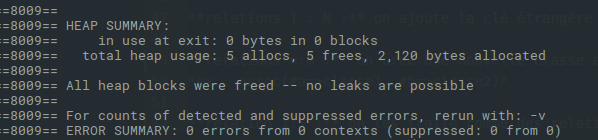
\includegraphics[width=8cm]{leak_summary.png}
\end{figure}


Concernant l'organisation du travail, nous avons réussi à bien nous répartir les tâches. Les fonctions creerElement et creerListe on été faites en TP, de même que le début de insererElement. Océane s'est chargée de débugger cette dernière et de la compléter, ainsi que de faire les fonctions rechercherElement et tableau\_vide. Louis s'est chargé de faire les fonctions supprimerElement, supprimerListe, fusionnerListes, afficher et menu. Ces fonctions ont été débuggées par Océane et le main.c fait par nous deux. La partie de test a aussi été faite par nous deux, et il en va de même pour le rapport. 
Pour aider à l'organisation du travail, nous avions décidé de faire le TP sur Github afin de pouvoir y accéder facilement durant les vacances. 

\end{document}



























